\chapter{Contexto}

    Com o objetivo de fazer a extração de micro-serviços de uma arquitetura monolítica, é necessário em primeiro lugar, entender a filosofia de cada uma das arquiteturas, os seus benefícios e desafios inerentes pelo modo como são estruturadas e o seu impacto no processo desenvolvimento de \textit{software}.

\section{Monólitos}

    Muitas das aplicações \textit{web} com as quais interagimos na atualidade são aplicações desenhadas segundo uma arquitetura monolítica. 
    
    Este estilo arquitetural é caracterizado por uma aplicação composta por toda a lógica fulcral relativa ao domínio do problema, contida num único processo. Este tipo de arquiteturas é tipicamente responsável por lidar com toda a funcionalidade relativa a persistência e manipulação de dados de acordo com o domínio de negócio. A camada mais externa, poderá também ser responsável por servir a interface para interação com o utilizador, ou, expor a sua funcionalidade através de uma API.
    
    Embora descrito como um estilo arquitetural pouco modular relativamente a uma arquitetura de micro-serviços, a sua modularidade é alcançada recorrendo a técnicas subjacentes da programação, como abstrações, implementações e extensões, permitindo assim a modularidade essencial a processos de \textit{refactoring} e adição de novas funcionalidades.
    
    Inerente à forma como esta arquitetura é estruturada, podem ser extraídas algumas vantagens da sua utilização: desenvolvimento rápido e simples no início no projeto; simplicidade no processo de \textit{deploy} dado a existência de um único componente; simples de escalar horizontalmente, sendo apenas necessário realizar cópias do monólito e colocá-las por de trás de um \textit{load balancer}.
   
   % todo REVER
    As vantagens referidas são especialmente apelativas quando se inicia um projeto, se trata de um projeto de curta duração, ou de baixa complexidade, no entanto, para outras situações é fundamental o pensamento a longo prazo em especial por ser estimado que cerca de 50\% do custo de desenvolvimento de \textit{software} é alocado para a manutenção \citep{software_maintenance_cost_alija_17}. Representando uma percentagem tão significativa do custo do projeto, manter o \textit{software} apto a adição de funcionalidade e correções é um dos principais desafios com o qual os \textit{developers} se deparam dado o crescente tamanho e complexidade do código. O \textit{deploy} apesar de mais simples em termos processuais, em atualizações do \textit{software} exige o \textit{re-deploy} da aplicação por completo. O facto do \textit{deploy} ser feito relativo a um único processo, que, em caso de falha num dos módulos da aplicação, poderá propragar a falha por todo o processo tornará a aplicação pouco fiável e resiliente a falhas.
    
    De um modo geral, arquiteturas monolíticas acompanhadas de boas práticas de desenho a nível estrutural, que procurem diminuir dependências e manter o acoplamento a um nível baixo são suficientes para lidar com um vasto conjunto de soluções \textit{standard}. A maior parte das desvantagens está associada ao processo de \textit{deploy}, à forma como lidam com falhas e à falta de flexibilidade quando se pretende realizar mudanças em estados avançados do projeto. 
    
%    \todo{ Há info interessante do Martin Fowler para adicionar}
    
    % Limitado relativamente ao conjunto de tecnologias
    % Problemas de dependências, versões, etc. (quando são necessário usar 2 versões diferentes na mesma app)
    % Promover mudanças localmente
    % Preferir designs pouco acoplados
    % Encapsulamento, etc
    

\section{Micro-serviços}

    % https://dzone.com/articles/microservices-vs-soa-whats-the-difference

    Descrito por \cite{fowler14_definition_microservices}, como uma arquitetura aplicacional composta por um conjunto de pequenos serviços, sendo cada um independente e auto-contido, executado no seu processo, com o objetivo de realizar bem um pequeno conjunto de tarefas. Com o seu isolamento, advém a necessidade de uma camada de comunicação. Tipicamente cada um dos serviços expõe a sua API, a qual receberá pedidos HTTP e responderá de acordo com a lógica definida no serviço.
    
    Inspirado na arquitetura SOA (\textit{Service Oriented Architecture}), que tem como objetivo lidar com algumas das dificuldades presentes em gerir arquiteturas monolíticas de elevada complexidade fragmentando a aplicação em vários serviços, deu-se continuidade à mesma filosofia de fragmentação da aplicação. Embora numa granularidade mais fina,  e pretendendo-se partilhar o mínimo possível entre micro-serviços. O princípio da responsabilidade única é um dos principais focos na definição da segregação dos serviços.
    
    
    \subsection{Vantagens}
    
        As vantagens dos micro-serviços são variadas comparativamente a arquiteruas monolíticas. Diversas das vantagens associados aos micro-serviços são resultantes das características adoptadas de sistemas distribuídos e do levar a um maior extremo a filosofia de arquiteturas orientadas a serviços. 
    
    \subsubsection*{Heterogenidade de tecnologias}
    
        A comunicação entre micro-serviços é feita tipicamente por HTTP recorrendo a uma tecnologia totalmente independente da linguagem, sendo uma das mais populares as APIs \textit{REST (Representational State Transfer)} que servem informação geralmente por \textit{Json (JavaScript Object Notation} ou \textit{XML (eXtensible Markup Language)}. Desta forma poderá haver uma variedade de tecnologias presente na \textit{stack} tecnológica da aplicação. Se determinado serviço necessitar de melhorias de performance, a alteração para uma tecnologia que permita trabalhar a mais baixo nível e otimizar a funcionalidade de um serviço específico, não terá impacto no restante sistema a nível funcional, desde que a estrutura da sua exposição para os restantes micro-serviços se mantenha igual. 
    
    \subsubsection*{Flexibilidade nos \textit{deploys}}
    
        Por mais reduzida que seja a alteração realizada sobre a aplicação, um sistema monolítico exige que o \textit{deploy} englobe toda a aplicação. Para diminuir o tempo de \textit{downtime} os \textit{deploys} são mais ponderados uma vez que não podem ser tão frequentes. No entanto, o acumular de alterações realizadas para \textit{deploy} de uma única vez trará um risco mais elevado pois será mais propício a erro. Várias alterações dificultam também a tarefa de identificar os eventuais problemas uma vez que estão abrangidos a vários componentes da aplicação.
    
        Contrariamente, os micro-serviços procuram manter uma relação próxima com a cultura de \textit{DevOps} e as filosofias de \textit{Continuous Integration (CI)} e \textit{Continuous Delivery (CD)}, filosofias que agilizam o processo de \textit{deploy}, por integrarem \textit{pipelines} automatizadas responsáveis por executar tarefas pré-definidas de verificação e validação do código, e consequentemente realizarem o \textit{deploy} para produção. Seguindo esta filosofia, os \textit{deploys} passam de pouco frequentes, contendo várias funcionalidades espalhadas por vários módulos, a muito frequentes, sendo cada \textit{release} estritamente associado ao seu serviço. \textit{Deploys} frequentes e específicos a um serviço, reduzem o risco, diminuem o \textit{downtime} e permitem mais facilmente identificar a origem dos problemas que cheguem a produção \citep{newman2015microservices}.
    
        \textit{Deploys} frequentes permitem ainda acompanhar mais naturalmente os ciclos de vida de metodologias ágeis, que dão grande importância à constante interação e \textit{feedback} com cliente e utilizadores finais. 
    
    
    \subsubsection*{Escalável}
       
       Quando se pretende escalar uma aplicação monolítica por necessidade apresentada por determinado módulo, toda a aplicação terá de ser também escalada. O nível de granularidade para escalar uma aplicação deste género, é bastante elevado, e como tal, bastante ineficiente, resultando num enorme desperdício de recursos computacionais e custos extra. Em contraste, os micro-serviços permitem uma escalabilidade de granularidade consideravelmente fina, proporcionando a escalabilidade apenas dos serviços que estão sobre sobrecarga. Deste modo, haverá uma maior eficiência dos recursos em utilização e redução de custos.
       
       A granularidade fina de serviços, permite também otimizações a nível arquitetural. Por exemplo, um serviço que tenha elevadas taxas de escritas e leituras na base de dados, e o qual, por regras de negócio, não necessite de disponibilizar sempre a versão mais recente, pode ser separado para dois micro-serviços: o primeiro englobará a lógica já implementada e tratará das escritas, sendo que o segundo servirá apenas os dados periodicamente atualizados pelo primeiro. Este tipo de fragmentações permite aumentar a velocidade das leituras uma vez que a quantidade de \textit{locks} à base de dados será reduzido significativamente. Este segundo serviço poderá também recorrer a uma base de dados de tecnologia diferente que beneficie de melhores tempos de consultas.
       
    
    \subsubsection*{Resiliente e tolerante a falhas}
        
       Lidar com falhas, especialmente quando se trata de um sistema de grandes dimensões, é inevitável. Os micro-serviços, por seguirem uma abordagem de sistemas distribuídos, permitem isolar e limitar as falhas a determinadas secções da aplicação, contrariamente ao que aconteceria numa aplicação monolítica, em que a falha numa funcionalidade pode resultar na falha completa de toda a aplicação.
       A transição de uma arquitetura monolítica para uma de micro-serviços não resolve por si só todos estes problemas automaticamente, \cite{behara_2018_resilient_ms}, numa fase inicial, os micro-serviços estarão particularmente vulneráveis a falhas, dada a adição da comunicação pela rede ser mais propensa a falhas que a pura comunicação em memória. No entanto, o aumento de um único possível ponto de falha para vários é uma característica fundamental em tornar um sistema baseado em sistemas distribuídos resiliente e tolerante a falhas.
       
       Recorrendo a padrões como o \textit{Bulkhead}, analogia aos sistemas de impermeabilidade de navios, que permitem que a entrada de água no casco seja contida e isolada por compartimentos, é igualmente possível isolar falhas e manter o restante serviço funcional, recorrendo a grupos de serviços que serão auto-contidos, não afetando a disponibilidade dos restantes serviços, \cite{bulkhead_pattern}.
       
       
        
    
    \subsubsection*{Estrutura organizacional}
       
       O trabalho realizado por equipas de grandes dimensões em projetos complexos é por si só uma tarefa complexa e difícil de gerir. Habitualmente, as equipas são mantidas em grupos pequenos de elementos para facilitar essa gestão. Esta fragmentação em equipas alinha-se de uma forma natural com o que é expectável dos micro-serviços, \cite{newman2015microservices}, ou seja, o trabalho realizado por uma equipa será tipicamente associado a um segmento específico que estará representado por um conjunto reduzido de micro-serviços.  Segundo \cite{conwayslaw}, organizações que desenham sistemas, produzem sistemas que refletem a estrutura organizacional da própria organização. Existindo uma separação por equipas organizadas à volta do domínio de negócio e sua funcionalidade, otimiza-se e reduz-se a quantidade de canais de comunicação entre as diferentes equipas e diminui-se o impacto da estrutura organizacional no \textit{software}. 
       
       
    
    
\subsection{Desafios}   

    Vários dos desafios de utilização de micro-serviços são na realidade desafios inerentes do uso de sistemas distribuídos. Estes devem ser levados em conta no  \textit{design} de uma arquitetura de micro-serviços.
    
    % purpose
    % transactions
    % choreography
    
    % segregação
    % complexidade
    % comunicação dispendiosa
    
    A segregação dos vários serviços para diferentes processos obriga a uma comunicação pela rede, contrariamente ao que acontece nos monólitos, onde a comunicação entre componentes é realizada em memória. Recorre-se tipicamente a comunicações por \textit{HTTP} em \textit{APIs REST} ou a sistemas de comunicação assíncronos por mensagens (AMQP) \citep{communication_microservice_architecture_microsoft}.
    Este tipo de comunicação adiciona um \textit{overhead} que não será encontrado em aplicações monolíticas, exigindo a análise da sua utilização em componentes que necessitam de ter tempos de resposta muito curtos e têm como principal foco a realização de operações rapidamente.
    
   % \todo{o termo hostname talvez não seja o mais correto} 
    Numa fase inicial e em sistemas mais simples, o acesso a serviços será feito consultando ficheiros de configuração compostos pelas respetivas localizações dos serviços que permitirão um acesso simples e direto ao serviço pretendido, no entanto, com o objetivo de lidar com falhas e escalar automaticamente os serviços, surge a dificuldade em lidar com atribuições dinâmicas de \textit{hostnames} na rede. Recorre-se tipicamente à adição de uma camada extra de um \textit{discovery pattern} que tratará de identificar um serviço disponível para o qual o pedido será enviado \citep{richardson15_service_discovery}. A necessidade de adição deste padrão contribui para o aumento da complexidade da infraestrutura pela necessidade da sua correta configuração, pela adição de uma outra camada que tem de ser monitorizada e tida em conta quando há falhas na aplicação. 
    
    A identificação de \textit{bugs} e falhas pela realização de testes de alto nível, como por exemplo, testes \textit{end-to-end} e testes de integração, torna-se um processo mais complexo, visto que é necessário criar \textit{stubs} dos restantes serviços para garantir isolamento da fração que é testada relativamente ao restante sistema \cite{newman2015microservices}.
    
    Semelhantemente à realização de testes pelo sistema como um todo, a realização de \textit{debug} por vários serviços da aplicação é também dificultada, uma vez que há uma elevada quantidade de \textit{logs} criados pelos diferentes serviços \citep{nemer_19_summary}. A utilização de \textit{log aggregators} e outros sistemas é essencial para tentar mitigar este problema.
    
    % Estima-se que haja um aumento de 100ms por pedido (procurar referencia?)
    % os principais desafios são desafios de sistemas distribuidos
    % ver documentação Engenharia Web
    
    
\section{Grafos de Dependências}

    O uso de grafo de dependências é crucial no processo de identificar as ligações entre componentes para que posteriormente se possa processar com o intuito de definir quais as relações relevantes à proposta de extração de micro-serviços. Esta estrutura permitirá também posteriormente aplicar técnicas de \textit{slicing} para extrair e realizar o \textit{refactoring} com uma granularidade mais baixa contrariamente a uma manipulação das classes como um todo.
    
    O grafo de dependências mais relevante, por proporcionar a informação necessária à manipulação e \textit{sicling} do código é o \textit{System Dependence Graph (SDG)}. Um \textit{SDG} $G = (N,E)$ relativo a um programa $p$ é um digrafo em que os nodos em $N$ representam os \textit{statements} e predicados, e os \textit{edges} de $E$ representam as dependências entre eles \citep{graf10_sdg_generation, horwitz04_inter_procedural_slicing}. 
    De uma forma mais unitária os \textit{SDG} são composto por \textit{procedure/program dependence graphs (PDG)} que por sua vez são compostos por \textit{control flow graphs (CFG)} e \textit{data flow graphs (DDG)}. O \textit{CFG} representa as dependências de fluxo entre os \textit{statements} e o \textit{data flow graph (DDG)} representa as dependências de dados entre os \textit{statements}.
    
    Diz-se que um nodo $n$ é \textit{control dependent} do nodo $m$, se a avaliação do nodo $m$ controlar se $n$ é executado (ex. quando $m$ é uma estrutura condicional que avalia a execução de $n$). De forma semelhante, $n$ é \textit{data dependent} em $m$, se o $n$ poder utilizar um valor calculado por $m$ \citep{graf10_sdg_generation}. Um exemplo de um \textit{PDG} pode ser observado na \textbf{Figura \ref{fig:pdg}}.
    
    \begin{figure}[h]
     	\begin{center}
     		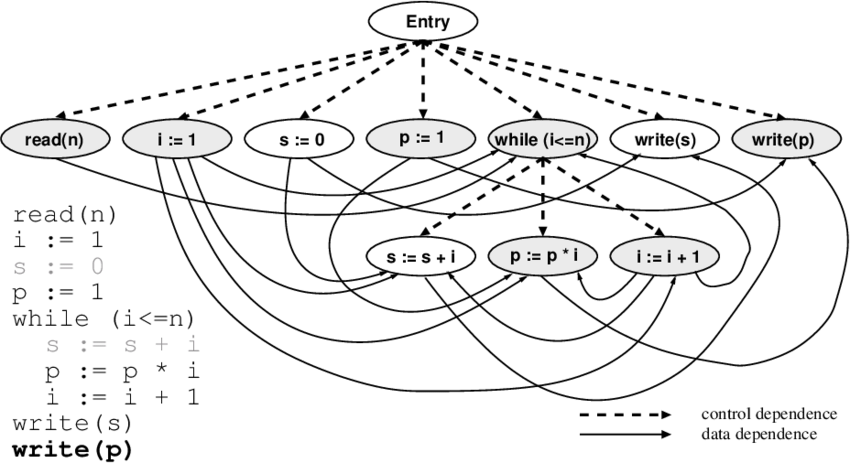
\includegraphics[width=\textwidth]{img/pdg.png}
     	\end{center}
     	\caption{\textit{Program dependence graph}}
     	\label{fig:pdg}
     	\floatfoot{Source: \cite{androutsopoulos10}}
 	\end{figure}
 	
 	A partir da composição dos \textit{PDG} que apenas fornecem informação intra-procedimental são adicionadas ligações que permitem identificar interações inter-procedimentais. Esta ligação é representada pela adição de ligações entre os \textit{call sites}, composto por nodos de invocação $c$ conectados ao procedimento invocado através de um \textit{call edge} $c \rightarrow _ce$ \citep{graf10_sdg_generation}. A passagem de parâmetros e retorno de resultados é definida por nodos \textit{actual-in} $a_i$ e \textit{actual-out} $a_o$ conectados ao seu respetivo nodo \textit{formal-in} $f_i$ ($a_i \rightarrow _{pi} f_i$) e \textit{formal-out} $f_o$ ($a_o \rightarrow _{po} f_o$) por um \textit{parameter-in} $p_i$ ou \textit{parameter-out} $p_o$. Este modelo de passagem de parâmetros garante que as ações inter-procedimentais são propagadas de volta à invocação do procedimento \citep{graf10_sdg_generation}. Um exemplo do \textit{SDG} com as respetivas ligações inter-procedimentais (\textit{actual-in} $\rightarrow$ \textit{formal-in}) pode ser observado na \textbf{Figura \ref{fig:sdg_exemplo}}.
    
     \begin{figure}[h]
     	\begin{center}
     		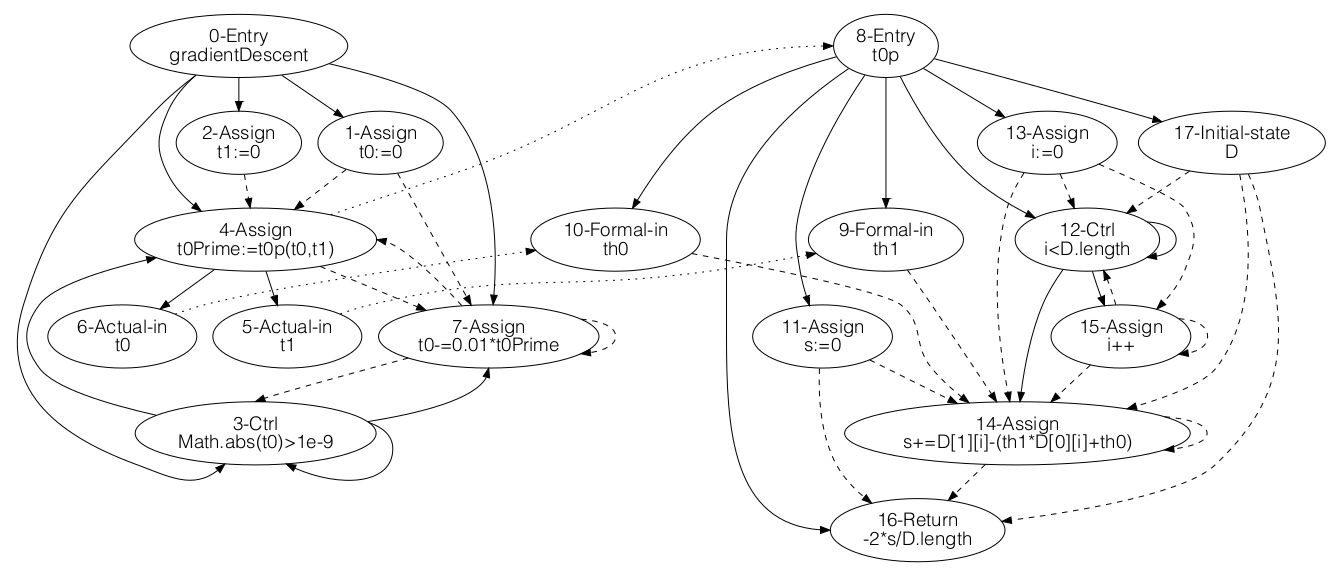
\includegraphics[width=\textwidth]{img/sdg_exemplo.png}
     	\end{center}
     	\caption{\textit{System Dependence Graph}}
     	\label{fig:sdg_exemplo}
     	\floatfoot{Source: \cite{marin18_sdg}}
 	\end{figure}
    

    
    % loosely coupled services
    
    
    

    
    
    
    
    
    
    